\RequirePackage{lineno}
%\documentclass[preprint,nofootinbib,showpacs,prl,superscriptaddress,secnumarabic,amssymb,nobibnotes,aps,floatfix]{revtex4}
\documentclass[twocolumn,nofootinbib,showpacs,prl,superscriptaddress,secnumarabic,amssymb,nobibnotes,aps,floatfix]{revtex4}
\usepackage{graphicx}
\usepackage{hyperref}
\usepackage{amsmath}
\usepackage{dcolumn}% Align table columns on decimal point
\usepackage{bm}% bold math
%
\def\Dirac#1{#1\hskip-5pt/}
%
\newcommand*\patchAmsMathEnvironmentForLineno[1]{%
\expandafter\let\csname old#1\expandafter\endcsname\csname #1\endcsname
\expandafter\let\csname oldend#1\expandafter\endcsname\csname end#1\endcsname
\renewenvironment{#1}%
{\linenomath\csname old#1\endcsname}%
{\csname oldend#1\endcsname\endlinenomath}}%
\newcommand*\patchBothAmsMathEnvironmentsForLineno[1]{%
\patchAmsMathEnvironmentForLineno{#1}%
\patchAmsMathEnvironmentForLineno{#1*}}%
\AtBeginDocument{%
\patchBothAmsMathEnvironmentsForLineno{equation}%
\patchBothAmsMathEnvironmentsForLineno{align}%
\patchBothAmsMathEnvironmentsForLineno{flalign}%
\patchBothAmsMathEnvironmentsForLineno{alignat}%
\patchBothAmsMathEnvironmentsForLineno{gather}%
\patchBothAmsMathEnvironmentsForLineno{multline}%
}


%
\begin{document}
\linenumbers

\title{First Exclusive Measurement of Deep Virtual Compton Scattering off $^4$He: Toward the 3D tomography of nuclei}

\newcommand*{\ANL}{Argonne National Laboratory, Argonne, Illinois 60439}
\newcommand*{\ANLindex}{1}
\affiliation{\ANL}
\newcommand*{\ORSAY}{Institut de Physique Nucl\'eaire, CNRS/IN2P3 and Universit\'e Paris Sud, Orsay, France}
\newcommand*{\ORSAYindex}{2}
\affiliation{\ORSAY}
\newcommand*{\JLAB}{Thomas Jefferson National Accelerator Facility, Newport News, Virginia 23606}
\newcommand*{\JLABindex}{3}
\affiliation{\JLAB}
\newcommand*{\ODU}{Old Dominion University, Norfolk, Virginia 23529}
\newcommand*{\ODUindex}{4}
\newcommand*{\INFNGE}{INFN, Sezione di Genova, 16146 Genova, Italy}
\newcommand*{\INFNGEindex}{5}
\newcommand*{\LPSC}{LPSC, Universit\'e Grenoble-Alpes, CNRS/IN2P3, Grenoble, France}
\newcommand*{\LPSCindex}{6}
\newcommand*{\UTFSM}{Universidad T\'{e}cnica Federico Santa Mar\'{i}a, Casilla 110-V Valpara\'{i}so, Chile}
\newcommand*{\UTFSMindex}{7}
\newcommand*{\MISS}{Mississippi State University, Mississippi State, MS 39762-5167}
\newcommand*{\MISSindex}{8}
\newcommand*{\VIRGINIA}{University of Virginia, Charlottesville, Virginia 22901}
\newcommand*{\VIRGINIAindex}{9}
\newcommand*{\VIRGINIATECH}{Virginia Polytechnic Institute and State University, Blacksburg, Virginia, 24061}
\newcommand*{\VIRGINIATECHindex}{10}

\newcommand*{\NOWJLAB}{Thomas Jefferson National Accelerator Facility, Newport News, Virginia 23606}
\newcommand*{\NOWODU}{Old Dominion University, Norfolk, Virginia 23529}
 %%%%%%%%%%%%%%% END OF Latex Macros for institute addresses  %%%%%%%%%%%%%%%%%%%%%%%%% 

\author {M.~Hattawy}
\affiliation{\ANL}
\affiliation{\ORSAY}
\author {N.A.~Baltzell} 
\affiliation{\ANL}
\affiliation{\JLAB}
\author {R.~Dupr\'{e}} 
\email[corresponding author: ]{dupre@ipno.in2p3.fr}
\affiliation{\ANL}
\affiliation{\ORSAY}
\author {K.~Hafidi} 
\affiliation{\ANL}
\author{S.~Stepanyan}
\affiliation{\JLAB}
\author {S.~Bultmann} 
\affiliation{\ODU}
\author{R.~De~Vita} 
\affiliation{\INFNGE}
\author {A.~El~Alaoui} 
\affiliation{\ANL}
\affiliation{\UTFSM}
\author {L.~El~Fassi} 
\affiliation{\MISS}
\author{H.~Egiyan}
\affiliation{\JLAB}
\author{F.X.~Girod} 
\affiliation{\JLAB}
\author {M.~Guidal} 
\affiliation{\ORSAY}
\author{D.~Jenkins}
\affiliation{\VIRGINIATECH}
\author{S.~Liuti} 
\affiliation{\VIRGINIA}
\author{Y.~Perrin}
\affiliation{\LPSC}
\author {B.~Torayev} 
\affiliation{\ODU}
\author {E.~Voutier} 
\affiliation{\LPSC}
\affiliation{\ORSAY}



\collaboration{The CLAS Collaboration}
\noaffiliation

%
\date{\today}
\begin{abstract}
We report the first exclusive measurement of coherent deeply virtual 
Compton scattering off a nucleus for $A>1$. The experiment used the 6 GeV 
electron beam from the CEBAF accelerator at Jefferson Lab incident on a 
$^4$He gas target in the center of the CEBAF large acceptance spectrometer 
(CLAS). A specially designed radial 
time projection chamber (RTPC) was used to detect the recoiling $^4$He
nuclei and ensure the exclusivity of the process. The measured beam-spin 
asymmetries are larger than that observed on the proton in the same kinematic 
domain. Since $^4$He is a spin-zero target, we were able to extract, in a 
model-independent way, the real and imaginary parts of the $^4$He 
Compton form factors, $\cal H_A$, which are functions of the generalized parton 
distribution $H_A$. This pioneering measurement of coherent deeply virtual 
Compton scattering on the $^4$He nucleus, with a fully exclusive final state 
via nuclear recoil tagging, leads the way toward 3D imaging of the partonic 
structure of nuclei.
\end{abstract}
\pacs{Valid PACS appear here}

\maketitle 

Rich information on quantum chromodynamics (QCD) can be extracted from the 
internal structure of hadrons. In the recent past, development of the 
generalized parton distribution (GPD) framework has offered a possibility to 
obtain new information about the momentum and spatial degrees of freedom of the 
quarks and gluons inside hadrons 
\cite{Mueller:1998fv,Ji:1996ek,Ji:1996nm,Radyushkin:1996nd,Radyushkin:1997ki}.
In impact parameter space the GPDs are indeed interpreted as a tomography of 
the transverse plane for partons carrying a given fraction of the proton 
longitudinal momentum 
\cite{Burkardt:2000za,Diehl:2002he,Belitsky:2002ep,Burkardt:2005hp}. 

The most promising way to access GPDs experimentally is through the measurement 
of deeply virtual Compton scattering (DVCS), \textit{i.e.}, the hard exclusive 
electroproduction of a real photon.  While other processes are known to be 
sensitive to GPDs, the measurement of DVCS is considered the cleanest probe and 
has been the focus of efforts at Jefferson Lab, HERA, and CERN
\cite{Stepanyan:2001sm,Airapetian,Chekanov:2003ya,Aktas:2005ty,Chen:2006na,Munoz 
Camacho:2006hx,Girod:2007aa,Mazouz:2007aa,Gavalian:2009,Seder:2015,Pisano:2015,Jo:2015ema}.  
The vast majority of these measurements focused on the study of proton 
structure and allowed for an extraction of the three-dimensional image of the 
proton (for details on the formalism, see 
\cite{Goeke:2001tz,Diehl:2003ny,Ji:2004gf,Belitsky:2005qn,Boffi:2007yc,Guidal:2013rya}).
This framework is also applicable to nuclei, giving access to novel 
information about nuclear structure in terms of quarks and 
gluons \cite{Dupre:2015jha}.
Study of the 3D structure of nuclei appears to be especially important
in light of the large nuclear effects observed in nuclear parton distribution 
functions \cite{Geesaman:1995yd,Norton:2003cb,Hen:2016kwk}.

\begin{figure}[tb]
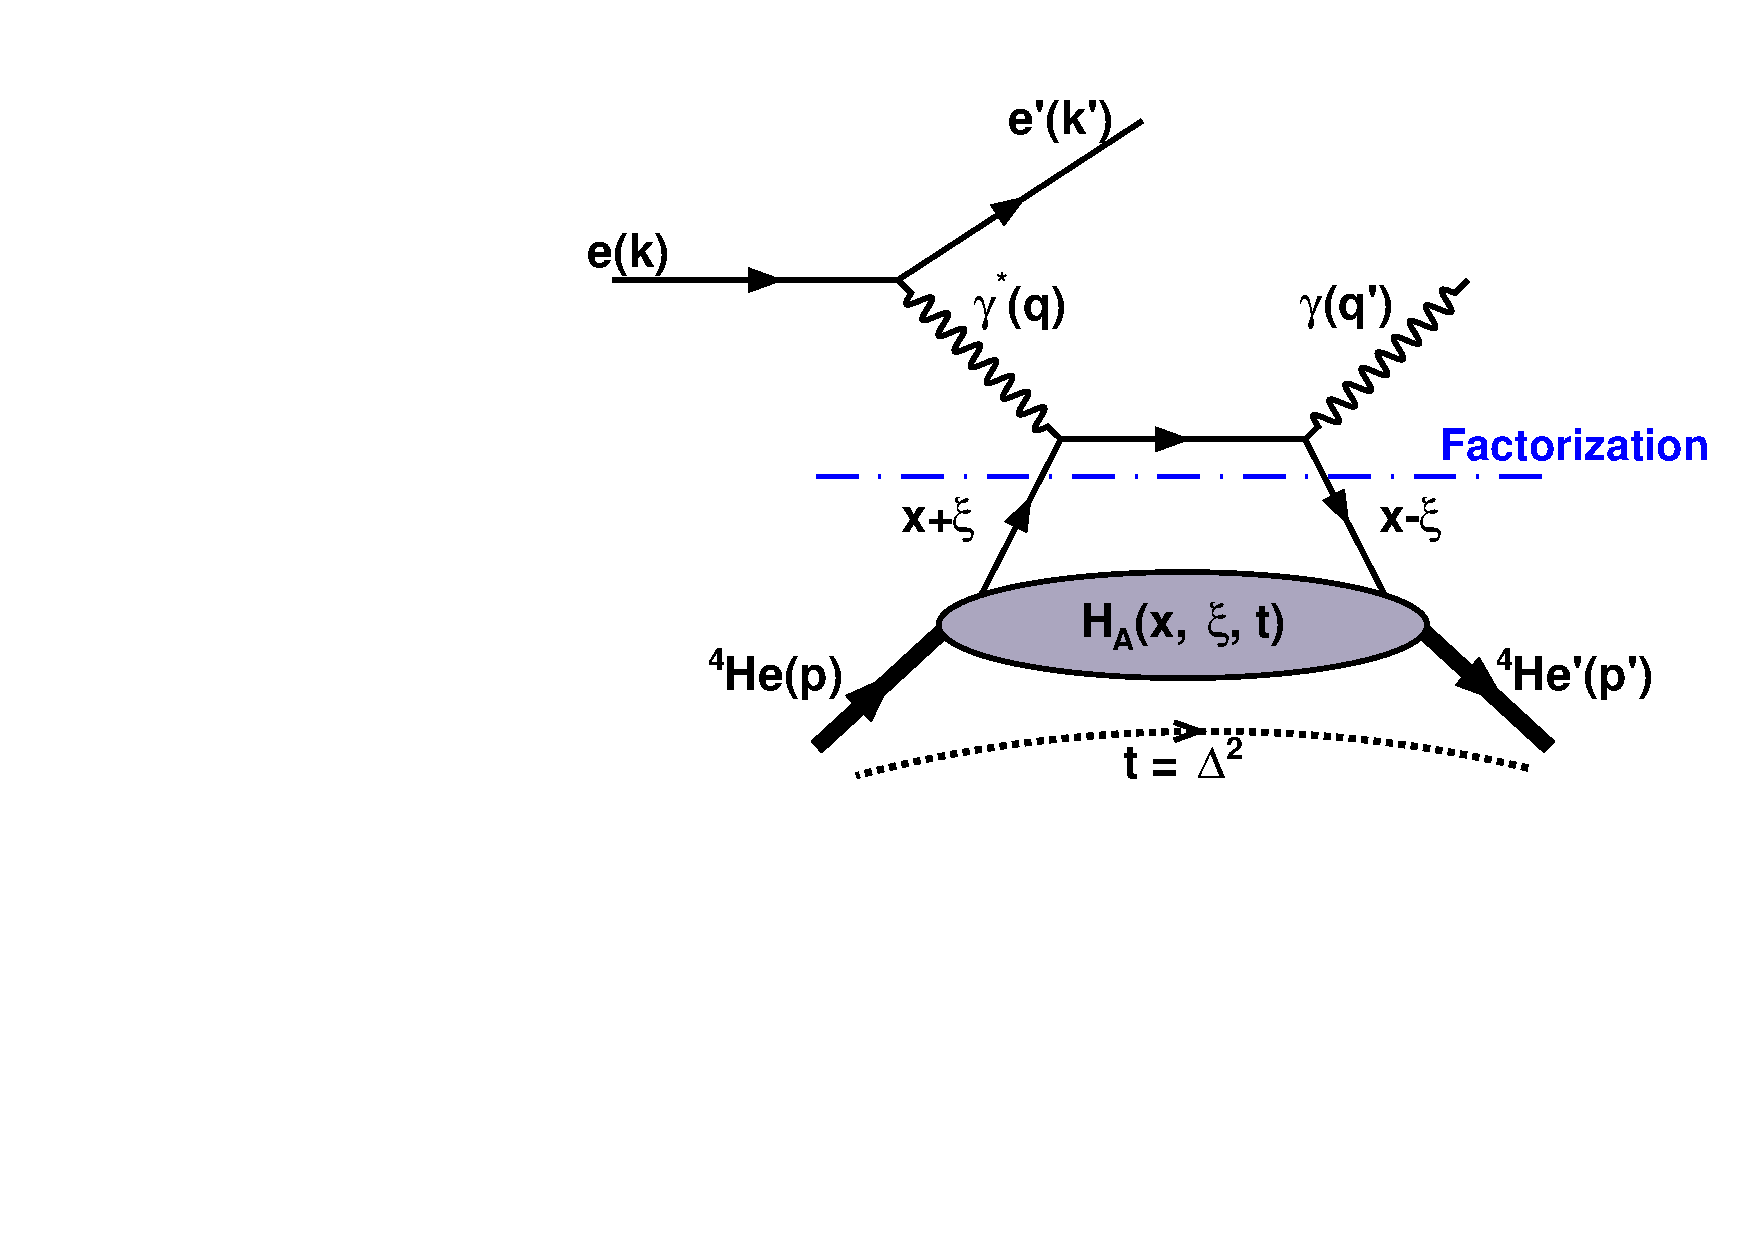
\includegraphics[width=6.5cm]{figs/DVCS_diagram.pdf}
\caption{Representation of the leading-order handbag diagram of the DVCS 
process off $^4$He.}
\label{fig:diags}
\end{figure}

One must overcome two major experimental challenges in measuring coherent 
nuclear DVCS, $eA\rightarrow e^\prime A^\prime\gamma$. First, the cross section 
of coherent scattering is suppressed due to the nuclear form factor, and 
second, the intact recoil nucleus ($A^\prime$) must be detected to ensure coherence.  
Fig.~\ref{fig:diags} illustrates the handbag diagram for coherent DVCS on 
$^4$He, where four-vectors of the electrons, photons, and $^4$He are denoted by
$k/k^\prime$, $q/q^\prime$, and $p/p^\prime$ respectively. For large virtual photon's 
4-momentum squared, $Q^2=-(k-k')^{2}$, and small squared momentum transfer, $t=(p-p')^{2}$, the DVCS handbag 
diagram can be factorized into two parts \cite{Freund_Collins,Ji_Osborne}. The 
hard part includes the photon-quark interaction and is calculable in 
perturbative QCD. The non-perturbative part is parametrized in terms of GPDs, 
which embed the partonic structure of the hadron. The GPDs depend on the three 
variables $x$, $\xi$, and $t$ as introduced in Fig.~\ref{fig:diags}. The 
parameter $\xi$ relates to the Bjorken variable $x_{B}$: $\xi\approx 
{{x_B}\over{2-x_B}}$, where $x_B=\frac{Q^2}{2M\nu}$, $\nu=k^0-k^{0\prime}$, and 
$M$ is the proton mass. The parameter $x$ is the quark's internal loop momentum 
fraction and cannot be accessed experimentally. We in fact measure 
Compton form factors (CFF) \cite{Guidal:2013rya}, which are
complex amplitudes defined as:

\begin{align}
\begin{split}
\Re e(&\mathcal{H}_{A}) = \\
    &\mathcal{P} 
\int_{0}^{1}dx[H_A(x,\xi,t)-H_A(-x,\xi,t)] \, C^{+}(x,\xi), 
\end{split} \\
\Im m(&\mathcal{H}_{A}) = H_A(\xi,\xi,t)-H_A(-\xi,\xi,t),
\end{align}
with $H_A$ the GPD, $\mathcal{P}$ 
the Cauchy principal value integral, and $C^{+}(x,\xi)$ a coefficient function 
($=  \frac{1}{x-\xi} + \frac{1}{x+\xi}$).

Until now, the only available data on nuclear DVCS was from the HERMES 
experiment \cite{Ellinghaus:2002zw}, where coherence in the reaction was based 
only on kinematic cuts on the measured scattered electron and real photon. The 
measurement was performed on a large set of nuclei ($^4$He, N, Ne, Kr and Xe), 
but contamination from incoherent processes could influence the
measurement significantly \cite{Guzey:2003jh}. Accordingly, direct detection 
of the low-energy recoil nucleus is critical in guaranteeing the nucleus 
remains intact. 

The $^4$He nucleus is an ideal experimental target for DVCS on nuclei, as it 
is light enough to be detected in such a setting, while it is subject to 
significant nuclear effects~\cite{JSeely} and has a spin-0. A helium target leads to another 
important advantage, as the number of GPDs defined for a hadron depends on its 
spin. The structure of a spin-zero nucleus, such as $^4$He, is parametrized by 
only one chiral even GPD ($H_{A}(x,\xi,t)$) at leading twist, while 4 GPDs 
arise in the nucleon case. This significantly simplifies the interpretation of 
the data and allows a model independent extraction of the $^4$He CFF 
($\mathcal{H}_{A}$) presented at the end of this letter. 

The CEBAF large acceptance spectrometer (CLAS) in Hall-B at Jefferson Lab has been
previously used successfully for DVCS measurements on the nucleon
\cite{Girod:2007aa,Gavalian:2009,Seder:2015,Pisano:2015,Jo:2015ema}.  In order
to extend its capabilities to nuclear DVCS with a fully exclusive final state,
we built a specialized radial time projection chamber (RTPC) for the detection
and identification of low-energy recoiling light nuclei. 
The experiment E08-024 took place in Hall-B at Jefferson Lab in 2009 using the 
nearly 100\% duty factor, longitudinally polarized electron beam (83$\%$ 
polarization) at an energy of 6.064 GeV. The data were collected over 40 days 
using a 6 atm gaseous $^4$He target placed 64 cm upstream of the nominal center 
of CLAS. For DVCS experiments, the CLAS 
baseline design~\cite{Mecking:2003zu} 
is supplemented with an inner calorimeter (IC) and a solenoid magnet. The IC 
extends the photon detection acceptance of CLAS to polar angles as low as 
4$^{\circ}$. The 5 T solenoid magnet has two functions; it provides the magnetic 
field for the momentum analysis in the RTPC, and at the same time acts as 
the guiding field for the low-energy M\o{}ller electrons, that are absorbed in a  
heavy shield placed around the beam line. 

In our kinematics, the recoil $^4$He nuclei produced in DVCS have low momentum,
averaging 300 MeV/c. CLAS cannot detect such low-energy $\alpha$ 
particles, so in order to ensure the exclusivity of the measurement, we built a 
small and light RTPC to complement CLAS. The RTPC is a $20$-cm-long cylinder 
with a diameter of $15$ cm, positioned directly around the $^4$He gaseous 
target. The target is a $25$-cm-long and $6$-mm-diameter Kapton tube with 
$27$-$\mu$m-thick walls. The RTPC was calibrated specifically for the detection of 
$^4$He nuclei by utilizing elastic scattering $e^4$He$\to e^\prime$$^4$He with
a 1.2~GeV electron beam.


%\begin{figure}[tb]
%\vspace{-1.1cm}
%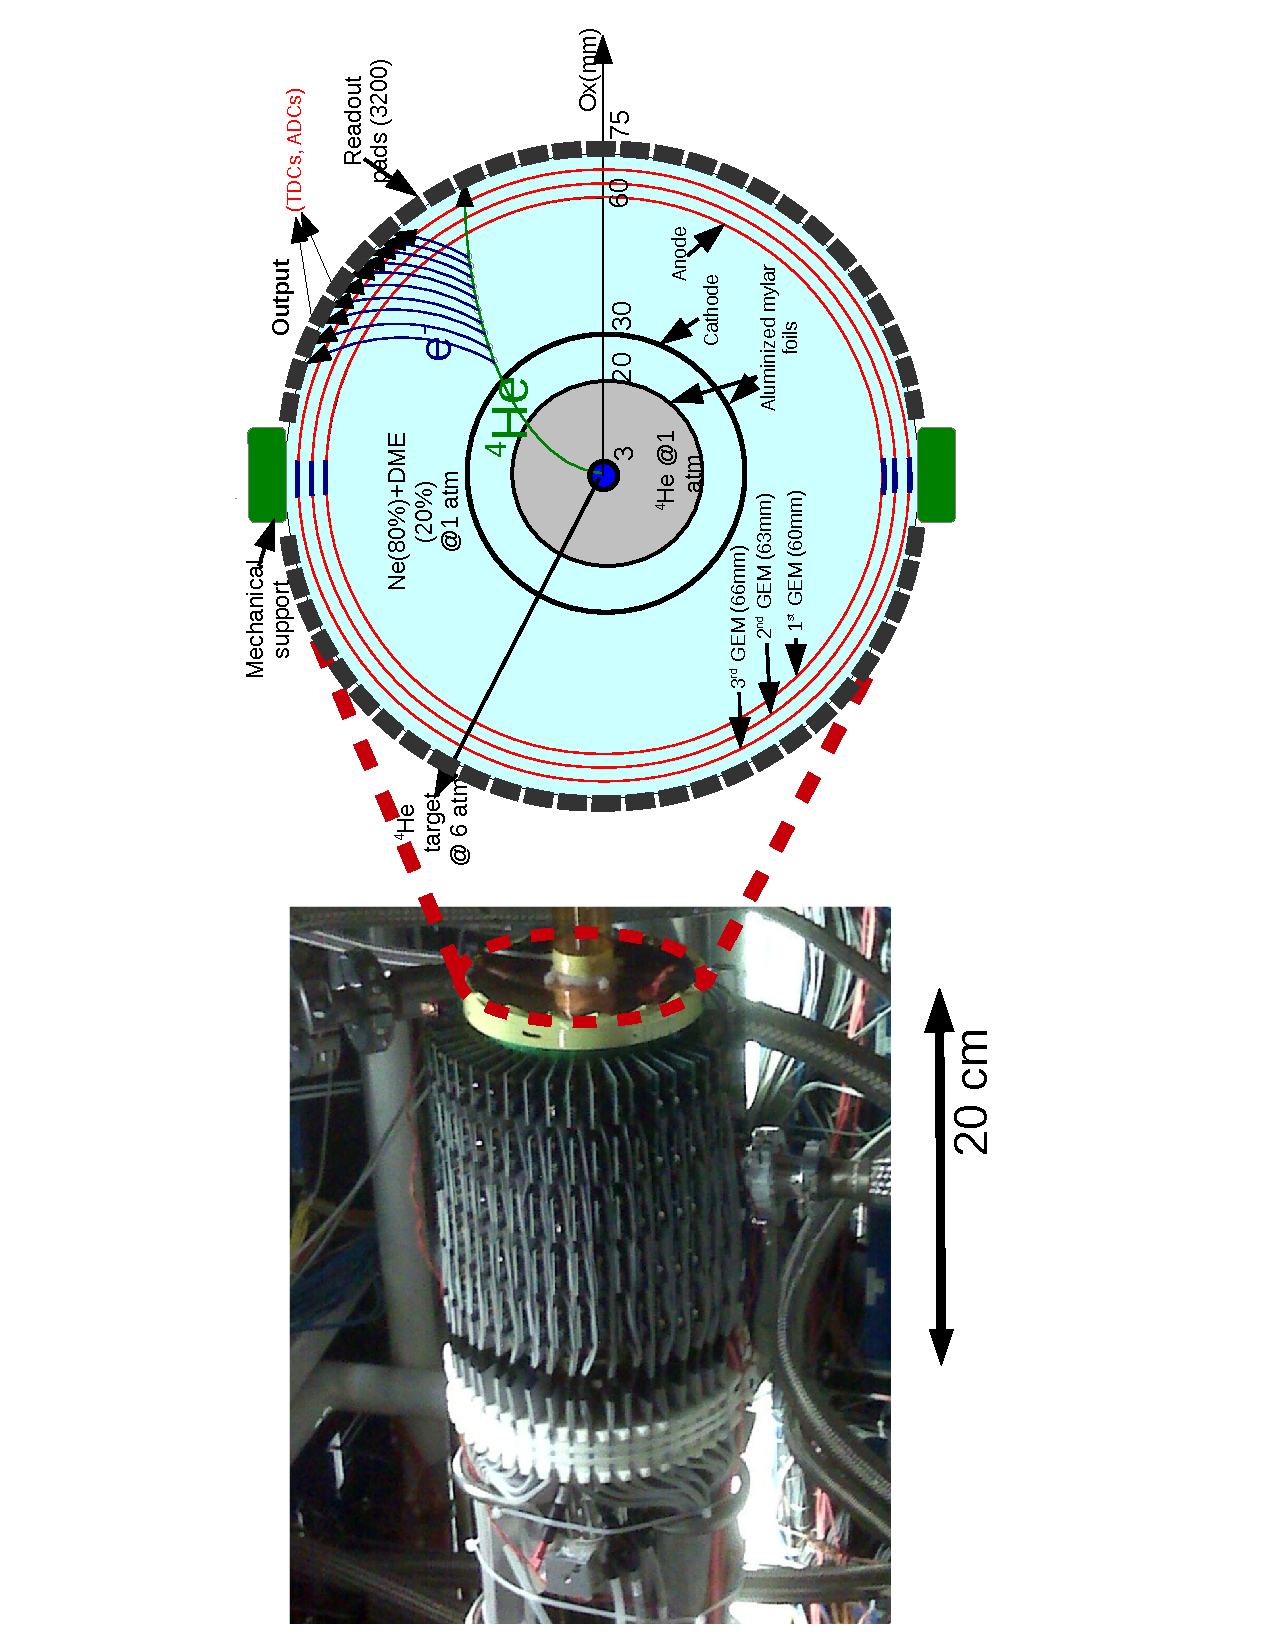
\includegraphics[width=6.5cm,angle=-90]{figs/RTPC.pdf}
%\vspace{-1.1cm}
%\caption{Left: A picture of the E08-024 RTPC before insertion into the 
%solenoid. Right: A cross section of the E08-024 RTPC perpendicular to the beam 
%direction. An illustration of a $^4$He track originating from the pressurized 
%straw target is shown along with the electrons produced in the drift region.}
%\label{fig:RTPC}
%\end{figure}

%DVCS selection
To identify coherent DVCS events, we first select events where one electron, 
one $^4$He, and at least one photon are detected in the final state. Electrons 
are identified using their measured momentum, time, and energy obtained from 
the CLAS drift chambers, \^{C}erenkov counters, scintillator counters, 
and electromagnetic calorimeters. The recoiling $^4$He nuclei are identified in 
the RTPC using time, track quality, and energy-loss cuts for tracks in the 
fiducial region \cite{Hattawy:thesis}. In addition, we apply a vertex-matching 
cut to ensure that the 
electron and helium nucleus originate from a common reaction vertex in the 
target cell. The photons are 
detected in either the IC or the CLAS electromagnetic calorimeter. Note that 
even though the DVCS reaction has only one real photon in the final state, 
events with more than one good photon are not discarded at this stage. These
are caused by accidental coincidences of soft photons that do not affect 
directly our measurement. We consider only the most energetic photon of an 
event as a DVCS photon candidate.
This prescription however slightly increases the corrections associated with
the $\pi^0$ and the accidental backgrounds discussed below. 

To ensure the interaction occurs at the partonic level and the DVCS handbag 
diagram is dominant, we select events with $Q^{2}$ greater than 1 
GeV$^{2}/$c$^{2}$. Exclusivity of the coherent DVCS reaction is optimized by 
applying a set of cuts on the following kinematic variables: the coplanarity 
angle $\Delta\phi$ between the ($\gamma,\gamma^*$) 
and ($\gamma^*$,$^4$He$'$) planes, the missing energy, mass, and transverse
momentum of the $e'^4$He$'\gamma$ system, the missing mass squared of 
the $e'^4$He$'$ system, and the angle $\theta$
between the measured photon and the missing momentum of the $e'^4$He$'$ system.  
The experimental data for the most relevant exclusivity observables and applied
cuts are shown in Fig.~\ref{fig:kin-cuts} (see \cite{Hattawy:thesis} for additional details).
%The most relevant of these cuts are presented in Fig.~\ref{fig:kin-cuts}, which 
%shows 3$\sigma$ cuts except for the missing energy (which appears to be too 
%large and for which we reduced the cut window to [-0.45,0.5] GeV).
We also 
reject events where a $\pi^0$ is identified by invariant mass reconstruction of 
two photons. About 3200 events pass these requirements, and their kinematic 
distributions are shown in Fig.~\ref{fig:kin-coverage}.

\begin{figure}[tb]
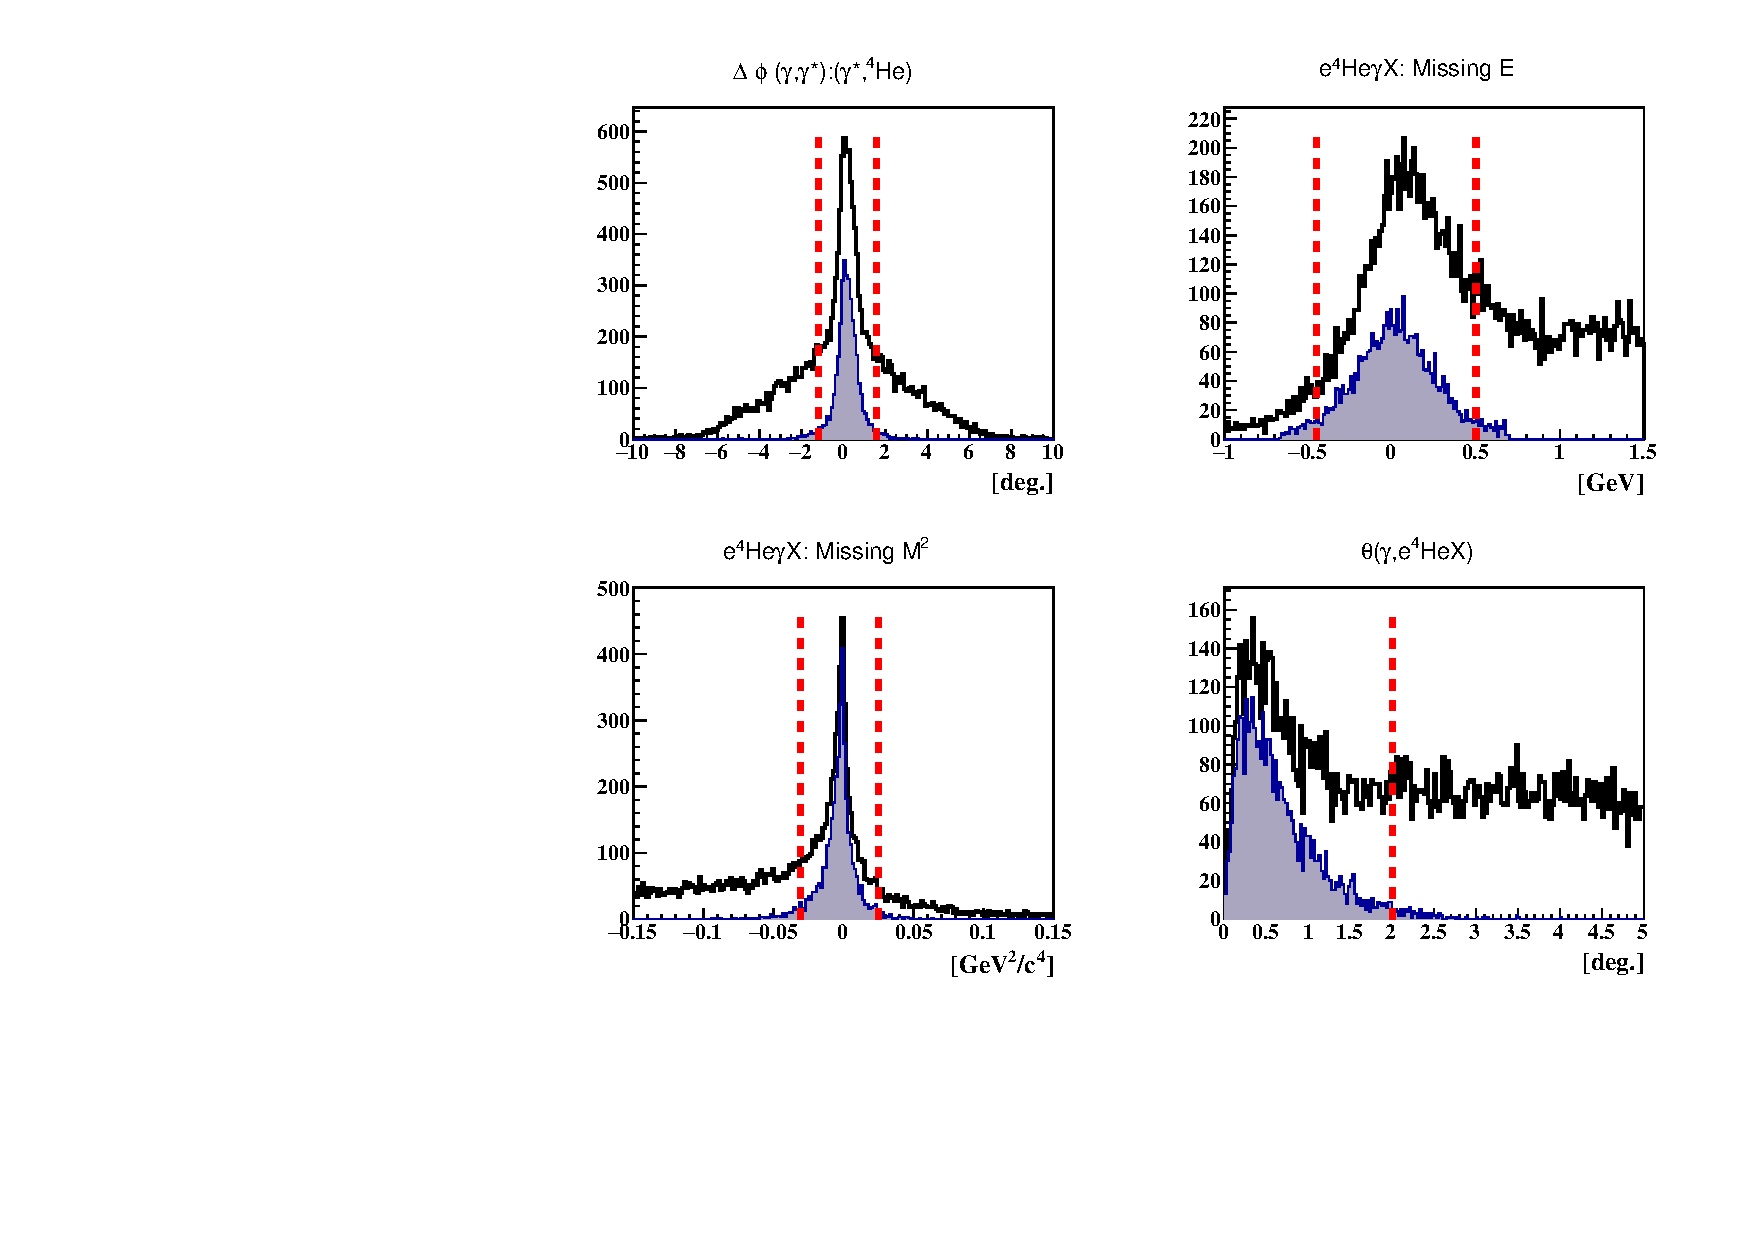
\includegraphics[width=9cm]{figs/coh_exc_cuts.pdf}
\caption{Four of the six coherent DVCS exclusivity cuts. The black 
distributions represent the initial candidate events, while the shaded 
distributions represent those which which passed all the exclusivity cuts except 
the quantity plotted. The vertical red lines represent the applied cuts.
The distributions from left to right and from top to bottom are: coplanarity 
angle $\Delta \phi$, missing energy $E_X$, missing-mass-squared $M_X^2$, and 
the cone angle $\theta$ between the measured photon and the missing momentum 
of the $e^\prime$He$^\prime$ system.}
\label{fig:kin-cuts}
\end{figure}
 

\begin{figure}[tb]
\hspace{-0.45cm}
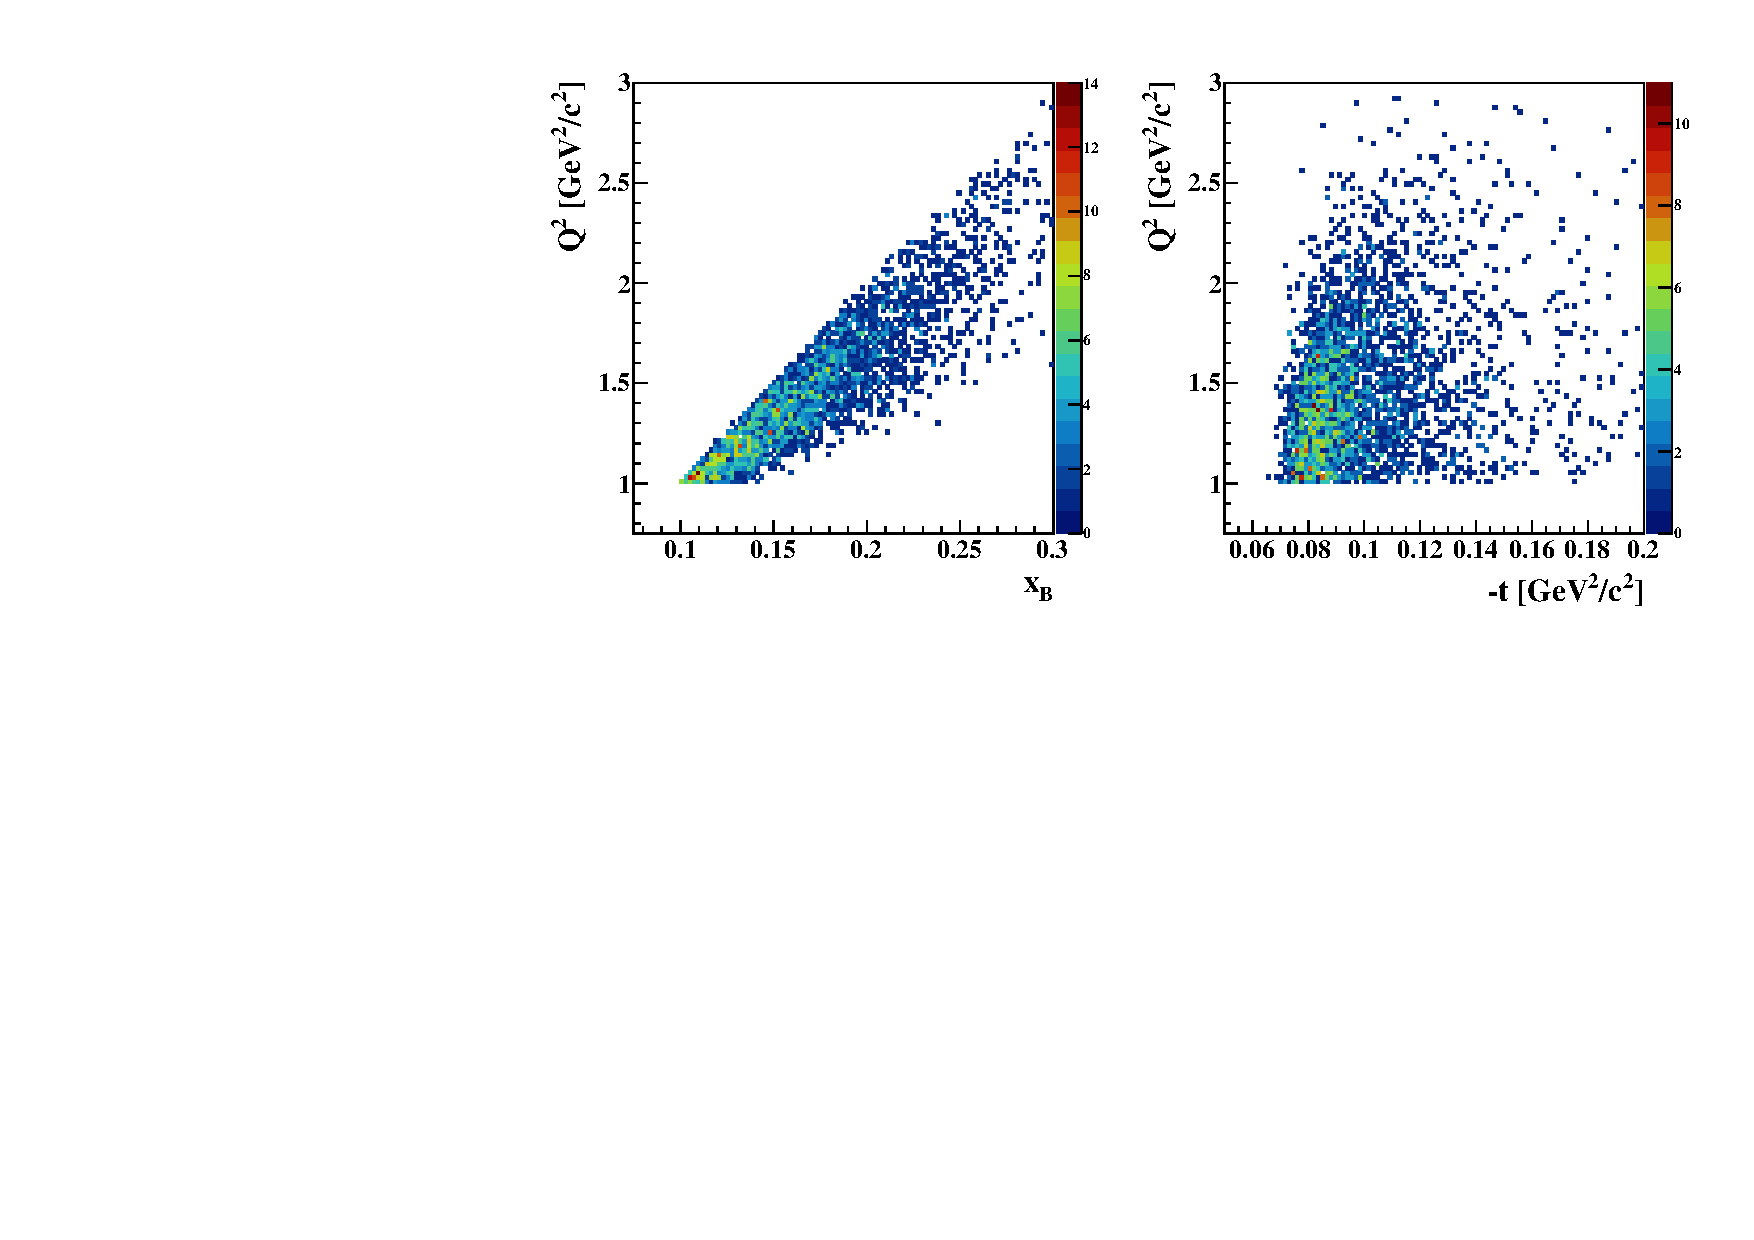
\includegraphics[width=8.5cm]{figs/Q2_xB_t_Coh.pdf}
\caption{Coherent DVCS event distributions for $Q^2$ after exclusivity cuts. 
The distributions are shown as a function of Bjorken variable $x_B$ (left) 
and as a function of squared-momentum transfer $-t$ (right).}
\label{fig:kin-coverage}
\end{figure}

%asymmetries
In this work, the physics observable extracted using coherent DVCS events is
the beam-spin asymmetry (BSA). The BSA on an unpolarized target, $A_{LU}$, is 
measured as the difference of cross sections for the reaction with opposite beam 
helicities normalized to the total cross section:
  \begin{equation}
  A_{LU} = \frac{d^{5}\sigma^{+} - d^{5}\sigma^{-} }
                {d^{5}\sigma^{+} + d^{5}\sigma^{-}},
    \label{BSA_equation}
  \end{equation}
where $d^{5}\sigma^{+(-)}$ is the DVCS differential cross 
section for positive (negative) beam helicity. 
In this ratio, luminosity normalization and
detector efficiencies largely cancel and $A_{LU}$ can be 
extracted from the reaction yields for the two helicities ($N^{+/-}$)
%expressed in terms of helicity-state yields ($N^{+/-}$)
\begin{equation}
A_{LU} = \frac{1}{P_{B}} \frac{N^{+} - N^{-}}{N^{+} + N^{-} },
\end{equation}
where $P_{B}$ is the degree of longitudinal polarization of the incident electron beam.

The DVCS and well-known Bethe-Heitler (BH) processes, in which the real 
photon is emitted by the incoming or the outgoing lepton, have the same final 
state and are indistinguishable. The amplitude of electroproduction of real
photons includes a sum of the amplitudes of these two processes. The BH 
amplitude is defined by the target form factors, while the DVCS amplitude is 
a combination of the form factors and GPDs. For our kinematics, the cross 
section of real photon electroproduction is dominated by the BH 
contribution, while the DVCS contribution is very small. However, the DVCS contribution is
enhanced in the observables sensitive to the interference term, {\it e.g.} 
BSA. The three terms entering the cross section calculation,
the square of the BH and DVCS amplitudes and their interference term, depend on the
azimuthal angle $\phi$ between the $(e,e^\prime)$ and $(\gamma^*,^4$He$^\prime)$ planes,
as shown for the nucleon in Ref.~\cite{Belitsky:2001ns} and for the spin-zero targets
in Refs.~\cite{Kirchner:2003wt,Belitsky:2008bz}. Based on this work, the BSA 
of a spin-zero hadron can be expressed as
\begin{equation}
\begin{split}
&A_{LU}(\phi) = \\
&\frac{\alpha_{0}(\phi) \, \Im m(\mathcal{H}_{A})}
{\alpha_{1}(\phi) + \alpha_{2}(\phi) \, \Re e(\mathcal{H}_{A}) + \alpha_{3}(\phi) \, 
\big( \Re e(\mathcal{H}_{A})^{2} + \Im m(\mathcal{H}_{A})^{2} \big)},
\end{split}
\label{eq:A_LU-coh}
\end{equation}
where $\Im m(\mathcal{H}_{A})$ and $\Re e(\mathcal{H}_{A})$ are the imaginary 
and real parts of the $^4$He CFF $\mathcal{H}_{A}$ and depend on the GPD $H_A$.  
Explicit expressions of the purely kinematic factors $\alpha_i$ are written in
Ref.~\cite{Belitsky:2008bz} and are functions of Fourier harmonics in the 
azimuthal angle $\phi$, the nuclear form factor $F_A(t)$, $Q^2$, $x_B$,
$x_{A} = \frac{x_{B}M_{N}}{M_{A}}$, $y=\frac{Q^{2}}{2x_{A}M_{A}E_{beam}}$, and 
$\epsilon = \frac{2x_{A}M_{A}}{\sqrt{Q^{2}}}$, where $M_{A}$($M_{N}$) is the $^4$He 
(nucleon) mass. Using the different $\sin(\phi)$ and $\cos(\phi)$ contributions, 
both imaginary and real parts of $\mathcal{H}_{A}$ can be extracted unambiguously
by fitting the $A_{LU}(\phi)$ distribution.

In this work, the azimuthal dependence of the beam-spin asymmetry has been studied 
for a wide range of kinematics ($Q^2$ between 1 and 2.2 GeV$^2$/c$^2$, $x_B$ between
0.1 and 0.3, and $-t$ between 0.07 and 0.16 GeV$^2$/c$^2$). We identified two main
backgrounds to our measurement, accidental coincidences and exclusive coherent
$\pi^0$ production.  The accidentals have particles originating from different events,
and we estimated their contribution to be 4.1\% of our sample. We evaluated this 
contribution by selecting events passing all our cuts but with an electron and 
helium originating from different vertices. The $\pi^0$ production can easily
be mistaken for DVCS when one of the two photons from the $\pi^0$ 
decay is produced at low energy in the laboratory frame and remains undetected.  
To estimate the effect of this background, we developed an event generator 
tuned on the experimental yield of exclusive $\pi^0$ measured by our 
experiment. We used this generator together with a GEANT3 simulation of our 
detector to estimate the ratio of the number of $\pi^0$ events where the 
two photons are detected to those that are misidentified as DVCS events. This 
ratio is then multiplied by the measured yield of exclusive $\pi^0$ events to 
correct the DVCS data.  Depending on the kinematics, we found contaminations of 
2 to 4\%. Studies of systematic uncertainties showed that the main contributions 
come from the choice of DVCS exclusivity cuts (8\% systematic uncertainty) and the 
large binning size (5.1\%), where the values are relative and quoted for $A_{LU}$
at $\phi=90^\circ$.  Added quadratically, the total systematic uncertainty
is about 10\% at $90^\circ$ (or 0.03, absolute), which is significantly smaller
than the statistical uncertainties in all kinematical bins. 

Due to limited statistics, dependence of the extracted asymmetries on the kinematical variables $Q^2$, 
$x_B$, and $t$ has been studied separately. In Fig.~\ref{fig:alu}, $A_{LU}$ for 
bins in each of the three variables is presented. The curves on the plots are fits with 
the function presented in Eq.~(\ref{eq:A_LU-coh}), where the real and imaginary 
parts of the CFF $\mathcal{H}_{A}$ are the free parameters of the fit.  In 
Fig.~\ref{fig:alu90} the $Q^2$, $x_{B}$, and $t$-dependencies of the fitted 
$A_{LU}$ at $\phi$~=~90$^{\circ}$ are shown. The $x_{B}$ and $t$-dependencies 
are compared to theoretical calculations by S.~Liuti and K.~Taneja 
\cite{simonetta_2}. The model accounts for the effect on the quark 
distribution of the virtuality (off-shellness) of the nucleon. The calculations are at slightly 
different kinematics than our data but still allow drawing some conclusions. The 
experimental results appear to have a larger asymmetries than the calculations. 
The difference may arise from the theoretical uncertainty in the determination 
of the crossing point where the parton nuclear distribution becomes larger than the 
nucleon one, and reverses the sign of the nuclear effect.

\begin{figure}[tb]
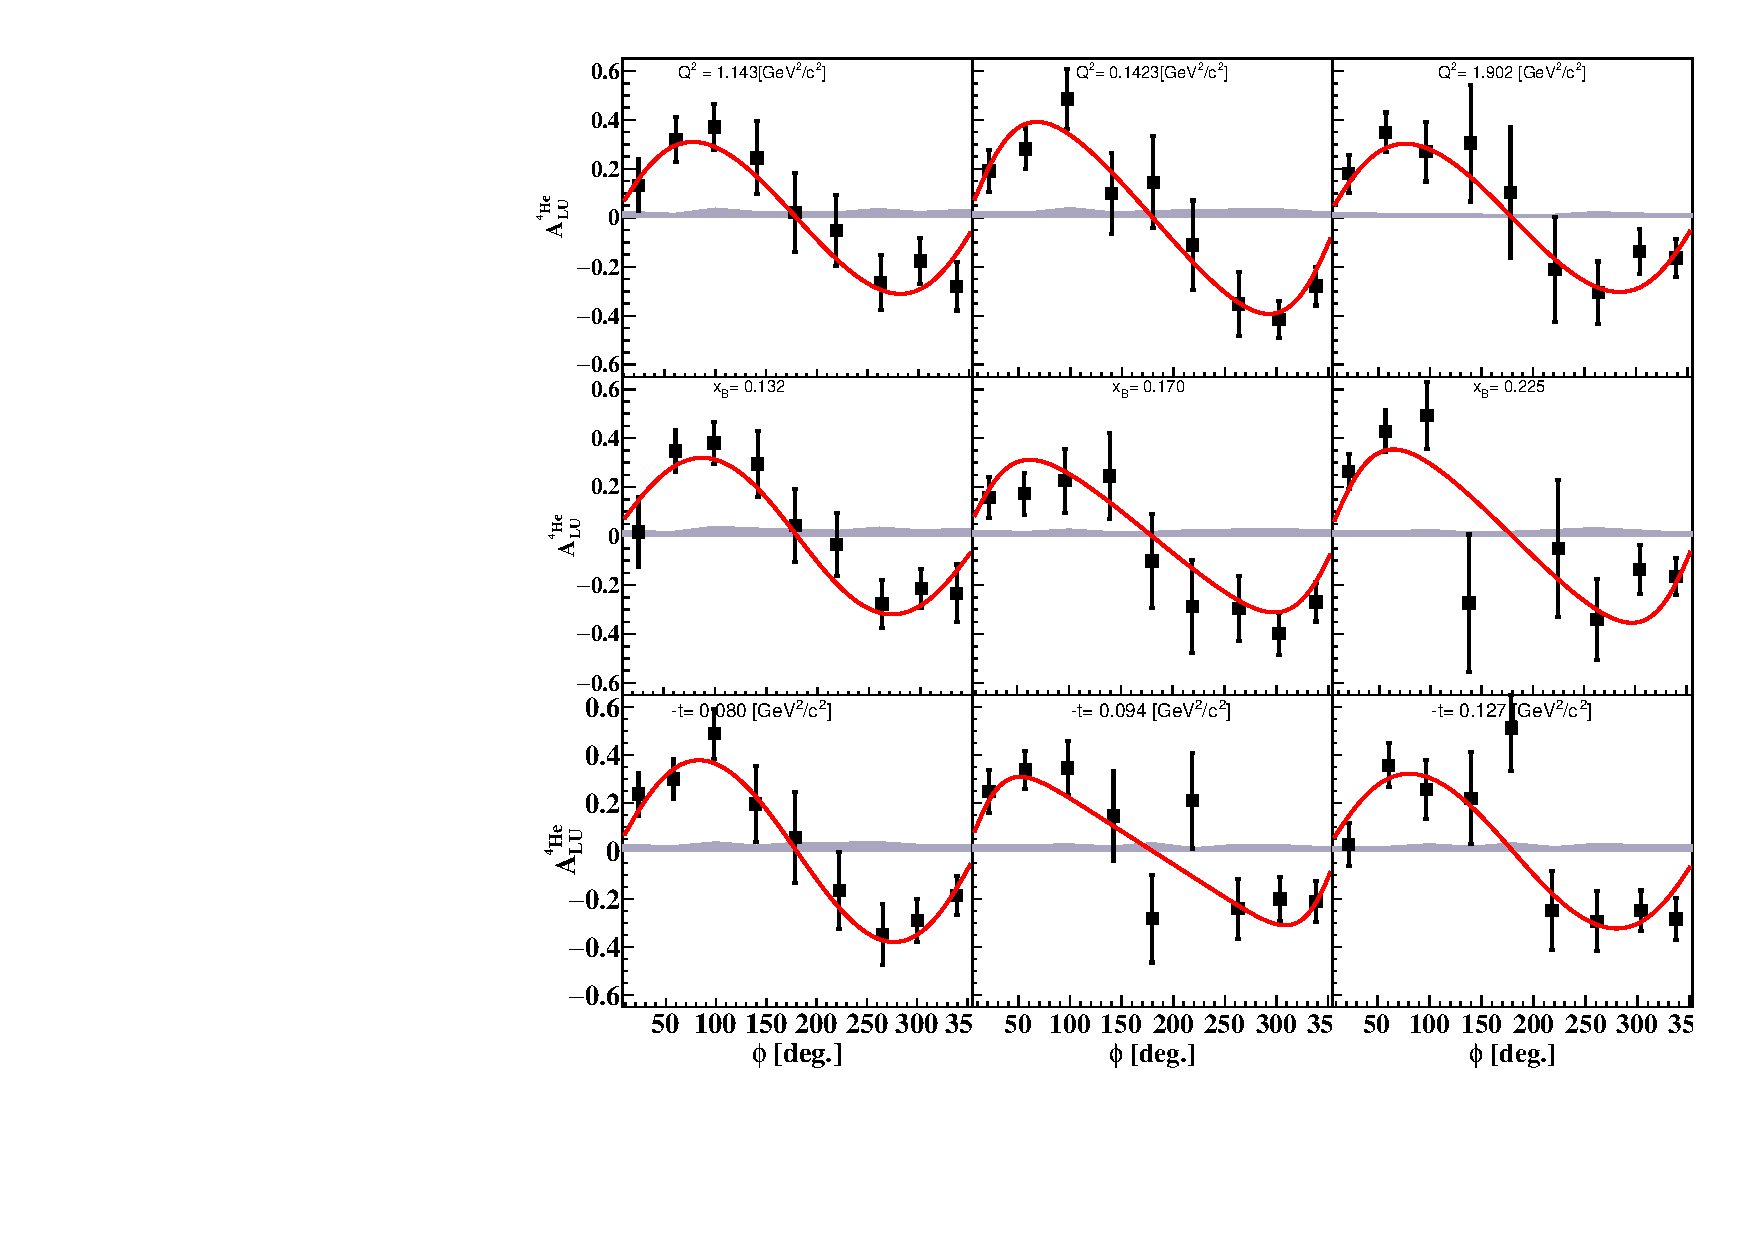
\includegraphics[width=8cm]{figs/coherent-ALU.pdf}
\caption{The coherent $A_{LU}$ as a function of azimuthal angle $\phi$. Results are presented
   for different $Q^{2}$ bins (top panel), $x_{B}$ bins (middle panel), and $t$ 
   bins (bottom panel).  The error bars represent the statistical 
   uncertainties. The gray bands represent the systematic uncertainties, 
   including the normalisation uncertainties. The red curves are the results of 
our fits with the form of equation \ref{eq:A_LU-coh}.}
\label{fig:alu}
\end{figure}

\begin{figure*}[tb]
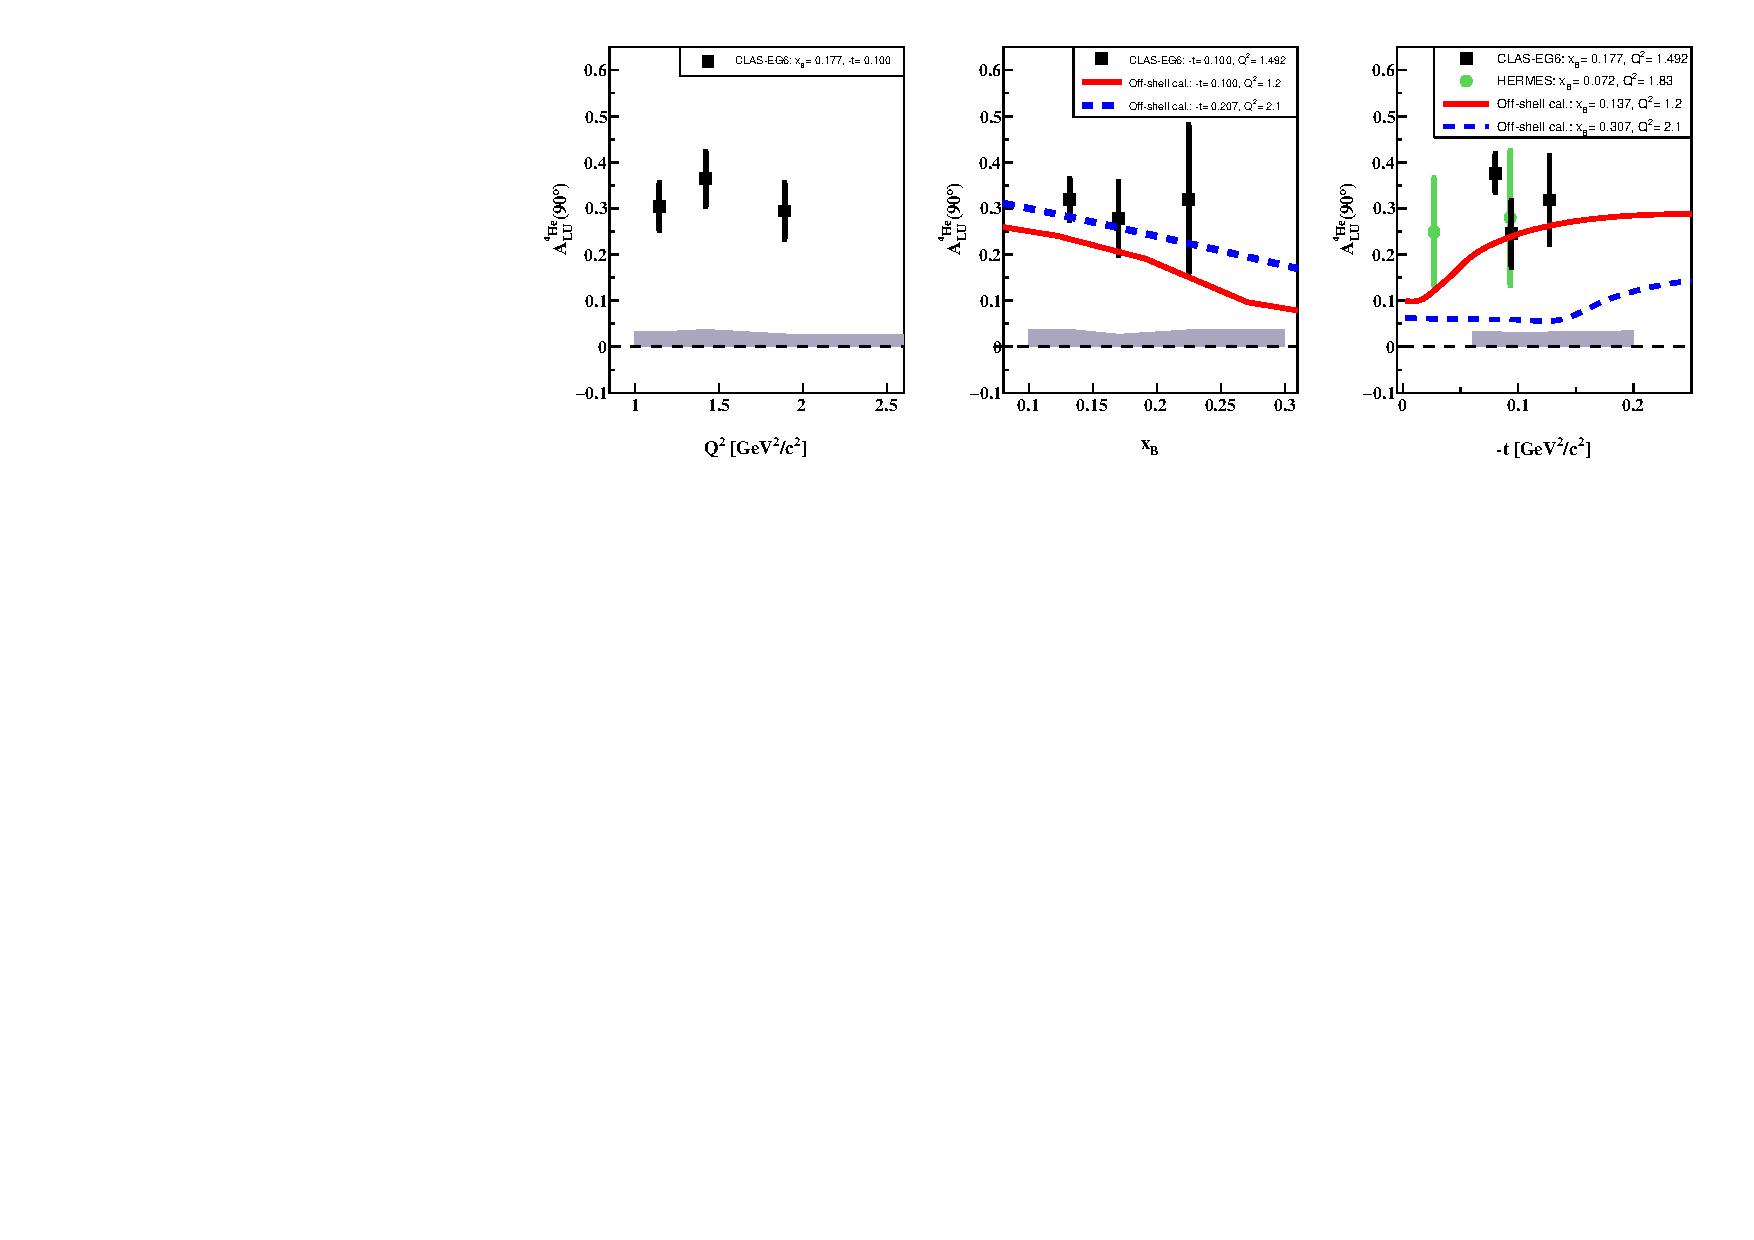
\includegraphics[width=17cm]{figs/coherent-ALU_90.pdf}
\caption{The $Q^{2}$ (left), $x_{B}$ (middle), and $t$-dependencies (right) of
   the $A_{LU}$ at $\phi$~=~90$^{\circ}$ (black squares). On the 
   middle plot: the full-red and the dashed-blue curves are theoretical 
   calculations from \cite{simonetta_2}. On the right: the green circles are 
   the HERMES $-A_{LU}$ (positron beam was used) inclusive measurements 
   \cite{Airapetian}, the colored curves represent theoretical calculations 
   from \cite{simonetta_2}.}
\label{fig:alu90}
\end{figure*}


\begin{figure}[tb]
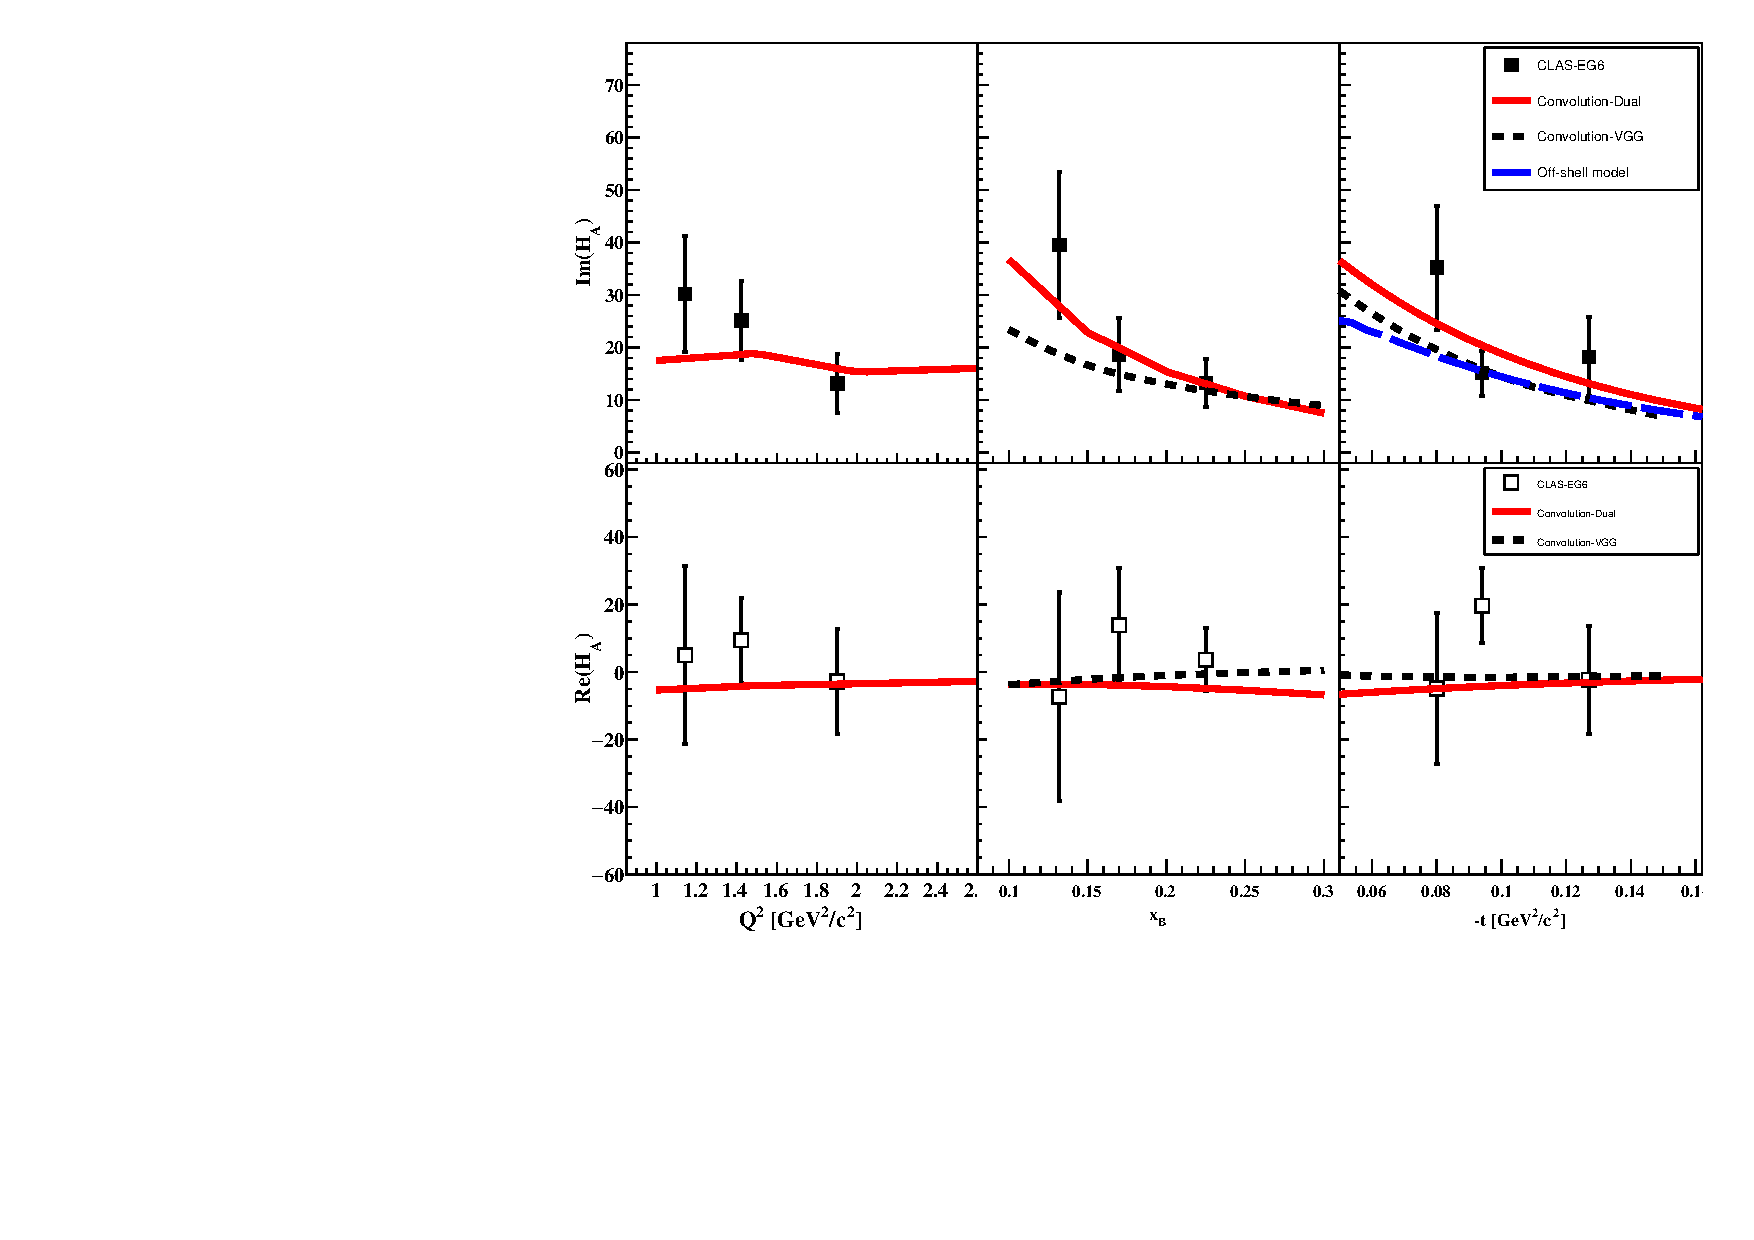
\includegraphics[width=8cm]{figs/Coherent_CFF.pdf}
\caption{The model-independent extraction of the imaginary (top panel) and
real (bottom panel) parts of the $^4$He CFF $\mathcal{H}_A$, as functions of
$Q^{2}$ (right panel), $x_B$ (middle panel), and $t$ (left panel). The full red 
curves are calculations based on an on-shell model from Ref.~\cite{Vadim_priv}.
The black-dashed curves are calculations from a convolution 
model based on the VGG model for the nucleons' GPDs \cite{Guidal_priv}. The 
blue long-dashed curve on the top-right plot is from
an off-shell model as described in Ref.~\cite{GonzalezHernandez:2012jv}.}
\label{fig:CFF_HA}
\end{figure}

The $Q^2$, $x_B$, and $t$ dependencies of the $^4$He CFF $\mathcal{H}_A$ 
extracted from the fit to the azimuthal dependence of $A_{LU}$ are shown in 
Fig.~\ref{fig:CFF_HA}. Curves on the graphs are model calculations, labelled 
{\it convolution} and {\it off-shell}. In the convolution model 
\cite{Vadim_priv}, the nucleus is assumed to be composed of non-relativistic 
nucleons, each interacting independently with the probe. The Convolution-Dual 
model is based on nucleon GPDs from the dual parametrization 
\cite{Guzey:2006xi}, where the Convolution-VGG uses nucleon GPDs  from the VGG 
model and is based on the double distributions ansatz \cite{DD_model}. The 
off-shell model is the same as in Fig.~\ref{fig:alu90} using an improved
GPD model for the nucleon \cite{GonzalezHernandez:2012jv}.

The results in Fig.~\ref{fig:CFF_HA} show that the extraction of the CFF
from the BSA is possible without any model dependent 
assumptions. The amplitude and the dependencies observed as a function of 
$Q^{2}$, $x_B$, and $t$ are in agreement with the theoretical expectations. One 
can see a difference between the precision of the extracted imaginary and real 
parts, this result is expected because of Eq.~(\ref{eq:A_LU-coh}) where 
$\alpha_2$ is much smaller than $\alpha_1$. While the precision of this 
measurement is not at a sufficient level to discriminate between the models, 
these results demonstrate the possibility of extracting the CFF of a spin 0 
target in a model independent way directly from a BSA measurement.


%conclusion
In summary, we present the first exclusive measurement of coherent DVCS off 
$^4$He using the CLAS spectrometer supplemented with a Radial Time Projection 
Chamber and a high pressure gaseous target. This setup allowed detection of the 
low energy $^4$He recoils in order to ensure an exclusive measurement of the
coherent DVCS process.
The azimuthal dependence of the measured BSA ($A_{LU}$) has 
been used to extract, in a model independent way, the real and the imaginary 
parts of the $^4$He CFF, $\mathcal{H}_A$. The extracted CFF is in  
agreement with predictions of the available models. This first fully exclusive 
experiment opens new perspectives for studying nuclear structure with the GPD 
framework and paves the way for future measurements at JLab using 12 GeV CEBAF 
and upgraded equipment.

%Acknowledgments

We acknowledge the staff of the Accelerator and Physics Divisions at Jefferson 
Lab for making this experiment possible. This work is supported by the U.S.  
Department of Energy, Office of Science, Office of Nuclear Physics, under 
contracts DE-AC02-06CH11357 and DE-AC05-06OR23177.

\begin{thebibliography}{99}

\bibitem{Mueller:1998fv} 
D. Mueller, D. Robaschik, B. Geyer, F.M. Dittes and J. Horejsi,
Fortsch.\ Phys. {\bf 42}, 101 (1994).
  
\bibitem{Ji:1996ek} 
X.D. Ji,
Phys.\ Rev.\ Lett. {\bf 78}, 610 (1997).

\bibitem{Ji:1996nm} 
X.D. Ji,
Phys.\ Rev.\ D {\bf 55}, 7114 (1997).

\bibitem{Radyushkin:1996nd}
A.V. Radyushkin,
Phys.\ Lett.\  B {\bf 380}, 417 (1996).

\bibitem{Radyushkin:1997ki} 
A.V. Radyushkin,
Phys.\ Rev.\ D {\bf 56}, 5524 (1997).

\bibitem{Burkardt:2000za} 
  M.~Burkardt,
  Phys.\ Rev.\ D {\bf 62}, 071503 (2000)
  Erratum: Phys.\ Rev.\ D {\bf 66}, 119903 (2002)

\bibitem{Diehl:2002he} 
  M.~Diehl,
  Eur.\ Phys.\ J.\ C {\bf 25}, 223 (2002)
  Erratum: Eur.\ Phys.\ J.\ C {\bf 31}, 277 (2003)
 
\bibitem{Belitsky:2002ep} 
  A.~V.~Belitsky and D.~Mueller,
  Nucl.\ Phys.\ A {\bf 711}, 118 (2002)

\bibitem{Burkardt:2005hp} 
  M.~Burkardt,
  Phys.\ Rev.\ D {\bf 72}, 094020 (2005)

\bibitem{Stepanyan:2001sm}
%S.~Stepanyan {\it et al.} [CLAS Collaboration],
S.~Stepanyan {\it et al.},
Phys.\ Rev.\ Lett. {\bf 87}, 182002 (2001).

\bibitem{Airapetian}
%A. Airapetian {\it et al.} [HERMES Collaboration],
A. Airapetian {\it et al.},
Phys.\ Rev.\ Lett. {\bf 87}, 182001 (2001);
JHEP {\bf 1207}, 032 (2012);
JHEP {\bf 1006}, 019 (2010);
JHEP {\bf 0806}, 066 (2008);
Phys.\ Lett.\ B {\bf 704}, 15 (2011);
Phys.\ Rev.\  D {\bf 75}, 011103 (2007);
JHEP {\bf 0911}, 083 (2009);
Phys.\ Rev.\ C {\bf 81}, 035202 (2010);
JHEP {\bf 1210}, 042 (2012).

\bibitem{Chekanov:2003ya}
%S. Chekanov {\it et al.} [ZEUS Collaboration],
S. Chekanov {\it et al.},
Phys.\ Lett.\  B {\bf 573}, 46 (2003).

\bibitem{Aktas:2005ty}
%A. Aktas {\it et al.} [H1 Collaboration],
A. Aktas {\it et al.},
Eur.\ Phys.\ J.\ C {\bf 44}, 1 (2005).

\bibitem{Chen:2006na} 
%S.~Chen {\it et al.} [CLAS Collaboration],
S.~Chen {\it et al.},
Phys.\ Rev.\ Lett.\ {\bf 97}, 072002 (2006).

\bibitem{Munoz Camacho:2006hx} 
%C. Mu\~noz Camacho {\it et al.} [Jefferson Lab Hall A Collaboration],
C. Mu\~noz Camacho {\it et al.},
Phys.\ Rev.\ Lett. {\bf 97}, 262002 (2006).

\bibitem{Girod:2007aa} 
%F.X. Girod {\it et al.} [CLAS Collaboration],
F.X. Girod {\it et al.},
Phys.\ Rev.\ Lett. {\bf 100}, 162002 (2008).

\bibitem{Mazouz:2007aa} 
%   M.~Mazouz {\it et al.} [Jefferson Lab Hall A Collaboration],
   M.~Mazouz {\it et al.},
   Phys.\ Rev.\ Lett.\  {\bf 99}, 242501 (2007)

\bibitem{Gavalian:2009} 
%G. Gavalian {\it et al.} [CLAS Collaboration],
G. Gavalian {\it et al.},
Phys.\ Rev.\ C {\bf 80}, 035206 (2009).

\bibitem{Seder:2015} 
%E. Seder {\it et al.} [CLAS Collaboration],
E. Seder {\it et al.},
Phys.\ Rev.\ Lett. {\bf 114}, 032001 (2015).

\bibitem{Pisano:2015} 
%S.~Pisano {\it et al.} [CLAS Collaboration],
S.~Pisano {\it et al.},
Phys.\ Rev.\ D {\bf 91}, 052014 (2015).

\bibitem{Jo:2015ema}
%H.~S.~Jo {\it et al.} [CLAS Collaboration],
H.~S.~Jo {\it et al.},
  Phys.\ Rev.\ Lett.\  {\bf 115}, no. 21, 212003 (2015)

\bibitem{Goeke:2001tz}
K. Goeke, M.V. Polyakov and M. Vanderhaeghen,
Prog.\ Part.\ Nucl.\ Phys. {\bf 47}, 401 (2001).

\bibitem{Diehl:2003ny}
M. Diehl,
Phys.\ Rept.  {\bf 388}, 41 (2003).

\bibitem{Ji:2004gf}
X.D. Ji,
Ann.\ Rev.\ Nucl.\ Part.\ Sci. {\bf 54}, 413 (2004).

\bibitem{Belitsky:2005qn}
A.V. Belitsky and A.V. Radyushkin,
Phys.\ Rept. {\bf 418}, 1 (2005).

\bibitem{Boffi:2007yc} S. Boffi and B. Pasquini,
Riv.\ Nuovo Cim. {\bf 30}, 387 (2007).

\bibitem{Guidal:2013rya} 
M.~Guidal, H.~Moutarde and M.~Vanderhaeghen,
Rept.\ Prog.\ Phys.\  {\bf 76}, 066202 (2013).

\bibitem{Dupre:2015jha} 
  R.~Dupr\'e and S.~Scopetta,
  Eur.\ Phys.\ J.\ A {\bf 52}, no. 6, 159 (2016)

\bibitem{Hen:2016kwk} 
  O.~Hen, G.~A.~Miller, E.~Piasetzky and L.~B.~Weinstein,
  arXiv:1611.09748 [nucl-ex].

\bibitem{Norton:2003cb} 
  P.~R.~Norton,
  Rept.\ Prog.\ Phys.\  {\bf 66}, 1253 (2003).

\bibitem{Geesaman:1995yd} 
  D.~F.~Geesaman, K.~Saito and A.~W.~Thomas,
  Ann.\ Rev.\ Nucl.\ Part.\ Sci.\  {\bf 45}, 337 (1995).

\bibitem{Freund_Collins}
A.~Freund and J.C.~Collins, 
Phys.\ Rev.\ D {\bf 59}, 074009 (1998)

\bibitem{Ji_Osborne}
X.-D.~Ji and J.~Osborne, 
Phys.\ Rev.\ D {\bf 58}, 094018 (1998)

\bibitem{Ellinghaus:2002zw}
%F.~Ellinghaus {\it et al.} [HERMES Collaboration],
F.~Ellinghaus {\it et al.},
AIP Conf.\ Proc.\  {\bf 675}, 303 (2003)

\bibitem{Guzey:2003jh} 
  V.~Guzey and M.~Strikman,
  Phys.\ Rev.\ C {\bf 68}, 015204 (2003)

\bibitem{JSeely}
J. Seely {\it et al.} 
Phys.\ Rev.\ Lett.\ {\bf 103}, 202301 (2009)

\bibitem{Mecking:2003zu} 
%B.~A.~Mecking {\it et al.} [CLAS Collaboration],
   B.~A.~Mecking {\it et al.},
   Nucl.\ Instrum.\ Meth.\ A {\bf 503}, 513 (2003).

\bibitem{Hattawy:thesis}
M.~Hattawy, Ph.D. thesis, Universit{\'e} Paris Sud - Paris XI, France 
[Institution Report No. 2015PA112161].

\bibitem{Belitsky:2001ns}
A.~V.~Belitsky, D.~Mueller and A.~Kirchner,
Nucl.\ Phys.\ B {\bf 629}, 323 (2002)

\bibitem{Kirchner:2003wt}
A.~Kirchner and D.~Mueller, 
Eur.\ Phys.\ J.\ C {\bf 32}, 347 (2003)

\bibitem{Belitsky:2008bz}
A.~V.~Belitsky and D.~Mueller,
Phys.\ Rev.\ D {\bf 79}, 014017 (2009)

%\bibitem{eg6_note}
%M. Hattawy {\it et al.} (CLAS-EG6 Working Group), CLAS internal analysis note, 
%2016.

\bibitem{simonetta_2}
S.~Liuti and K.~Taneja, 
Phys.\ Rev.\ C {\bf 72}, 032201 (2005)

\bibitem{Vadim_priv}
Private communications with V.~Guzey based on: 
V.~Guzey, Phys.\ Rev.\ C {\bf 78}, 025211 (2008).

\bibitem{Guzey:2006xi}
V.~Guzey and T.~Teckentrup,
Phys.\ Rev.\ D {\bf 74}, 054027 (2006)

\bibitem{Guidal_priv}
Private communications with M.~Guidal based on: 
M.~Guidal, M.~V.~Polyakov, A.~V.~Radyushkin and M.~Vanderhaeghen, 
Phys.\ Rev.\ D {\bf 72}, 054013 (2005).

\bibitem{DD_model}
I.~V.~Musatov and A.~V.~Radyushkin, 
Phys.\ Rev.\ D {\bf 61}, 074027 (2000).

\bibitem{GonzalezHernandez:2012jv}
J.~O.~Gonzalez-Hernandez, S.~Liuti, G.~R.~Goldstein and K.~Kathuria,
Phys.\ Rev.\ C {\bf 88}, no. 6, 065206, (2013).

\end{thebibliography}

\end{document}
